
\section{Methods}
All calculations reported in this study used a 5x5x1 supercell of graphene, 
as it was large enough to make inconsequential the interaction between periodic images of the adsorbed hydrogen atom and to assure that there are essentially unperturbed C atoms between the buckled regions in adjacent images in the $x$ and $y$ directions.
The geometries of graphene, both pristine and with a chemisorbed H atom, were provided by Kim et al.,\cite{10.1021/acsami.1c21821} and were obtained using the PBE+D3 DFT method.\cite{10.1063/1.3382344,10.1103/PhysRevLett.77.3865} 
For all systems, a vacuum spacing of \SI{16}{\angstrom} was used.

\subsection{Density functional theory calculations}
The single particle orbitals used in the trial wave functions for variational Monte Carlo (VMC) and DMC calculations were calculated using the PBE functional with the correlation consistent electron core potential (ccECP)\cite{10.1063/1.5040472,10.1063/1.4995643} pseudopotentials and a plane wave basis with an energy cutoff of 3,400 eV.
Monkhorst-Pack $k$-point grid meshes\cite{10.1103/PhysRevB.13.5188} were employed with a 13.6 meV Marzari-Vanderbilt-DeVita-Payne cold smearing of the occupations.\cite{10.1103/PhysRevLett.82.3296}
The PBE results were converged at a 6x6x1 $k$-point grid to 1 meV for graphene and graphene with an adsorbed hydrogen atom. The hydrogen atom trial was generated using a 1x1x1 $k$-point grid. Convergence studies can be found in Table S1 and S2 of the Supplementary Material.

In addition to the PBE calculations used to generate the trial wave functions for DMC, DFT calculations were carried out with the PBE0\cite{10.1063/1.478522} and Heyd–Scuseria–Ernzerhof (HSE) functionals\cite{10.1063/1.2404663} to determine if inclusion of exact exchange proves important for the adsorption energy.
Due to the inclusion of exact exchange, these calculations would be computationally prohibitive in a plane wave basis, particularly with the high energetic cutoff required by the ccECP pseudopotential.
For this reason, they were carried out all-electron with the POB-TZVP Gaussian type orbital (GTO) basis set.\cite{10.1002/jcc.23153}
Due to the use of GTOs, these calculations suffer from basis set superposition error (BSSE), which we corrected using Grimme's geometry-dependent counterpoise correction scheme.\cite{10.1063/1.3700154,10.1021/jp406658y} This correction resulted in a 113 meV reduction in the magnitude of the binding energy when using the PBE0 functional.
For the PBE0 and HSE calculations, a 12x12x1 $k$-point grid was used to assure binding energies converged to within 2meV.
Convergence data are supplied in Table S3 of the Supplementary Material.

The plane wave DFT calculations were carried out with the QUANTUM ESPRESSO version 6.3 code.\cite{10.1063/5.0005082,10.1088/0953-8984/21/39/395502,10.1088/1361-648X/aa8f79}
The Gaussian basis DFT calculations were carried out with CRYSTAL17,\cite{10.1002/wcms.1360,10.1063/5.0004892} save for the HSE calculation of the isolated hydrogen atom which was carried out using NWChem version 6.8\cite{10.1063/5.0004997} using the same basis as the calculations in CRYSTAL17.

\subsection{Quantum Monte Carlo calculations}
DMC is a projector quantum Monte Carlo (QMC) method, solving the Schr\"{o}dinger equation in imaginary time $\tau=it$; any initial state $\ket{\psi}$, that is not orthogonal to the true ground state $\ket{\phi_0}$ , will evolve to the ground state in the long time limit.
When dealing with Fermionic particles, the DMC method requires the use of the fixed-node approximation\cite{10.1063/1.440575} to maintain the antisymmetric property of the wave function. 
For efficient sampling and to reduce statistical fluctuations, we use a Slater-Jastrow trial wave function fixing the nodes through a Slater determinant comprised of single-particle orbitals, which, in this work, are expanded in a B-spline basis.
The Jastrow factor is a function that reduces the variance by explicitly describing dynamic correlation.
The Jastrow factor contains terms for one-body (electron-ion), two-body (electron-electron) and three-body (electron-electron-ion) interactions.
The one- and two-body terms were described with spline functions\cite{10.1109/MCSE.2010.122}, while the three-body terms were represented by polynomials.\cite{10.1103/PhysRevB.70.235119}
10 parameters were used for the one-body terms per atom type, and 10 parameters were employed per spin-channel for the two-body terms. The cutoffs on the one- and two-body terms were fixed to the Wigner-Seitz radius of the simulation cell.
The three-body terms were comprised of 26 parameters per term with a cutoff of 10 Bohr.
The parameters in the Jastrow factor were separately optimized for each geometry with the linear method\cite{10.1103/PhysRevLett.98.110201} using VMC.
To reduce the cost of the DMC calculations as well as to reduce the fluctuations near the ionic core regions, ccECP pseudopotentials were used to replace the core electrons.\cite{10.1063/1.5040472,10.1063/1.4995643}
The ccECP pseudopotentials were designed to be used with high-accuracy many-body methods.
\begin{figure}
    \centering
    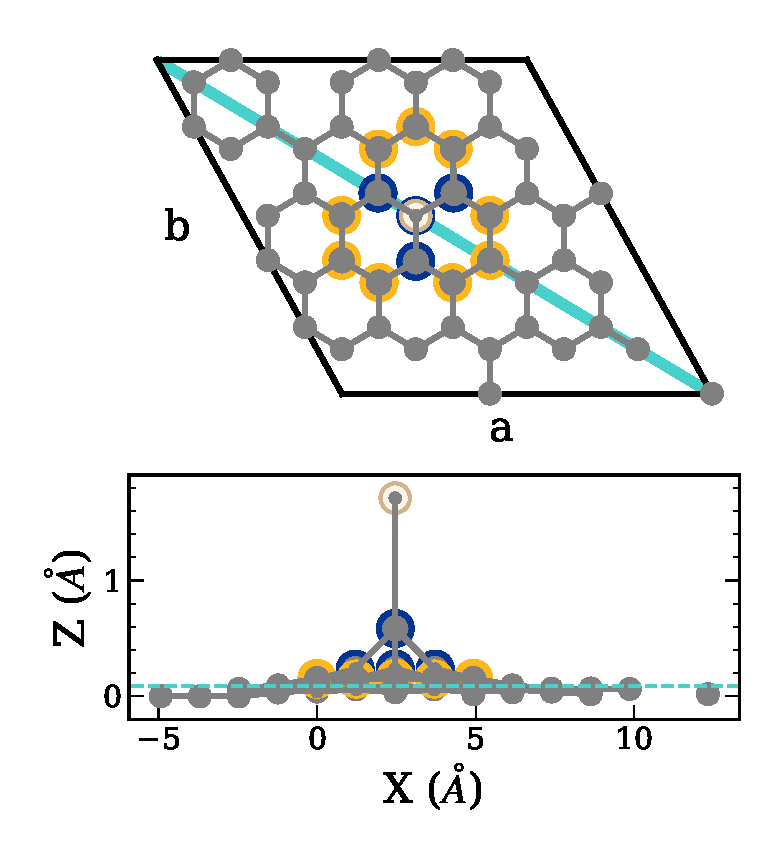
\includegraphics[width=\columnwidth,keepaspectratio]{Images/chapter4/hgraphene_python.eps}
    \caption{ Perpendicular view of the simulation cell (top) and a parallel view obtained by projection onto the $xz$-plane (bottom). The carbon atoms are colored gray and the hydrogen atom is denoted as white. For the perpendicular view, the cyan line represents the slice of the cell used to visualized electron density differences. For the parallel view, the dotted cyan line represents the mean carbon $z$ position. Blue outlined atoms are greater than one standard deviation away from the mean carbon $z$ position, whereas yellow atoms are between 0.5-1.0 $\sigma$.}
    \label{fig:cell}
\end{figure}
The non-local effects due to the pseudopotentials were addressed using the determinant-localization approximation along with the t-moves method (DLTM).\cite{10.1063/1.5119729, 10.1063/1.3380831}
Finite size effects were addressed using twist averaging.\cite{10.1103/PhysRevE.64.016702} The twist angles were chosen to be the symmetry unique points of the 6x6x1 $k$-point grid shifted by half a grid step away from the gamma point in each direction.

The DMC calculations were performed using the branching scheme proposed by Zen
et al. (ZSGMA)\cite{10.1103/PhysRevB.93.241118} with a population control target of 8,192 walkers and a time step of 0.005 a.u., which represented a balance between computational cost and finite timestep error in previous work.\cite{10.1103/PhysRevB.100.075430}



We define the binding energy as
\begin{equation}
E_b=E_{dgr+H}-(E_{gr}+E_{H})
\label{eq:binding}
\end{equation}
where $E_{dgr+H}$ is the energy of the distorted graphene sheet with a chemisorbed atomic hydrogen, $E_H$ is the energy of a hydrogen atom, and $E_{gr}$ is the energy of a pristine graphene sheet.
In the chemisorbed state, the hydrogen atom bonds directly over a carbon atom, causing this carbon to be pulled out of the sheet towards the hydrogen.\cite{10.1063/1.4896611,10.1126/science.aaw6378} 
The adjacent carbons are also pulled in the direction of the hydrogen leading to a distorted graphene sheet.


The QMC calculations were carried out using the QMCPACK code, with the workflow between QUANTUM ESPRESSO and QMCPACK managed by Nexus.\cite{10.1088/1361-648X/aab9c3,10.1063/5.0004860,10.1016/j.cpc.2015.08.012}
Figures~\ref{fig:cell} and \ref{fig:densdiff_dmcminusdft} were rendered with matplotlib\cite{10.1109/MCSE.2007.55} and the density plots were generated using VESTA.\cite{10.1107/S0021889811038970}
%%%%%%%%%%%%%%%%%%%%%%%%%%%%%%%%%%%%%%%%%%%%%%%%%%%%%%%%%%%%
